\documentclass[12pt]{article}

\usepackage{graphicx}
\usepackage{geometry}
\geometry{
	a4paper,
 	left=26mm,
 	right=26mm,
 	top=33mm,
 	bottom=38mm
}
\usepackage{color}
\definecolor{bluekeywords}{rgb}{0.13,0.13,1}
\definecolor{greencomments}{rgb}{0,0.5,0}
\definecolor{redstrings}{rgb}{0.9,0,0}

\usepackage{listings}
\lstdefinelanguage{FSharp}%
{morekeywords={let, new, match, with, rec, open, module, namespace, type, of, member, % 
and, for, while, true, false, in, do, begin, end, fun, function, return, yield, try, %
mutable, if, then, else, cloud, async, static, use, abstract, interface, inherit, finally },
  otherkeywords={ let!, return!, do!, yield!, use!, var, from, select, where, order, by },
  keywordstyle=\color{bluekeywords},
  sensitive=true,
  basicstyle=\ttfamily,
	breaklines=true,
  xleftmargin=\parindent,
  aboveskip=\bigskipamount,
	tabsize=4,
  morecomment=[l][\color{greencomments}]{///},
  morecomment=[l][\color{greencomments}]{//},
  morecomment=[s][\color{greencomments}]{{(*}{*)}},
  morestring=[b]",
  showstringspaces=false,
  literate={`}{\`}1,
  stringstyle=\color{redstrings},
}

\begin{document}


\begin{center}

{\large F\# Tutorial\\} \vspace{2mm}
\textbf{\LARGE Pipe-Forward Operator}\\
\vspace{1.5mm}
{\Large\emph{\today}}

\end{center}


\section{Syntax, variables, functions}

\subsection{Key concepts: } 

\begin{enumerate}
\item Having a good text editor helps you code much easier.
\item 
\begin{enumerate}
\item Once defined, a variable in F\# cannot change value (unless "mutable" is used)
\item If you need an updated value, create a new one.
\end{enumerate}
\item Different datatypes (e.g. integer and decimal-numbers) do not combine easily.
\item Defining and using functions in F\# is slightly different from math notation/ other languages.
\begin{enumerate}
\item F\# automatically detects the type of the variables (e.g. integer, double, etc.) for a function.
\item The variable types for a function will be enforced.
\end{enumerate}
\end{enumerate}

\subsection{Introduction: } 
\subsubsection{Comments}
You can use double-slash \texttt{//}, triple-slash \texttt{///}, or star-bracket \texttt{(* ...... *)} to make comments.

\begin{lstlisting}[language=FSharp]
// These words are ignored.
/// These words are ignored.
(* These words are ignored. *)
let x = 1
let y = x + 5
\end{lstlisting}

\vfill

\pagebreak

\subsubsection{Intellisense}
If you are using Visual Studio or Visual Studio Code, you can put your mouse on top of the variable name \texttt{x} or \texttt{y}, and see that it is an \texttt{int} or integer.

This feature will help you identify what is each variable/function, and make coding easier for you. 
\begin{center}
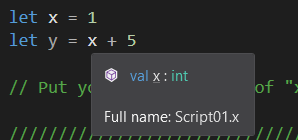
\includegraphics[width=5cm]{pictures/picture01.png}
\end{center}

\subsubsection{Common data types and printing}

Some of the common types in F\# are:
\begin{center}
\begin{tabular}{|c|c|c|}
\hline Keyword & Description & Print in output:
\\ \hline \texttt{int} & Integer & \texttt{\%i}
\\ \hline \texttt{double} or \texttt{float} & Decimal numbers & \texttt{\%f}
\\ \hline \texttt{string} & Words/Sentences & \texttt{\%s}
\\ \hline \texttt{bool} & True/False & \texttt{\%b}
\\ \hline - & Other objects & \texttt{\%A} or \texttt{\%O}
\\ \hline
\end{tabular}
\end{center}

\begin{lstlisting}[language=FSharp]
let name = "John"
let age = 21
let height = 170.5

printfn "My name is: %s" name
// Output:
// My name is: John

printfn "Name: %s. Age: %i. Height: %f." name age height
// Output:
// Name: John. Age: 21. Height: 170.500000

printfn "His height is: %.2f" height
// Output:
// His height is: 170.50
//// Show only two decimal.
\end{lstlisting}
For example, in the second example, inside the string-format, there are \texttt{\%s, \%i, \%f}. And so, we expect a string, integer, and decimal (in that order) after the string-format specification in order to completely print the result to the output console.

\vfill

\pagebreak

\subsubsection{Equality and simple if-else}

The \texttt{let ... = ...} combination is used to assigned a value to a variable. Other than this situation, the equal sign \texttt{=} is used for equality testing. \texttt{=, <>} are used for equality/inequality testing.


\begin{lstlisting}[language=FSharp]
let valueToTest = 20
let isValueEqualToTwenty = (valueToTest = 20)

if isValueEqualToTwenty then
    printfn "Yes, the value is Twenty"
else 
    printfn "No, the value is not Twenty"
// Output: "Yes, the value is Twenty"
///////////////////////////////////////

let inputUserName = "Jack"

if inputUserName = "John" then
    printfn "Welcome back, John"
else 
    printfn "Access denied."
// Output: "Access denied."
\end{lstlisting}

In Java/C++, \texttt{==, !=} are used for comparison, and in Javascript, \texttt{===, !==} are used.

\subsubsection{Immutability}

In F\#, variables are by default immutable/unchangable. Once defined, the value of a variable cannot be changed. You can make a variable changable/mutable using the keyword \texttt{mutable} and symbol \texttt{<-}, but this is \underline{highly discouraged}. (If you use VisualStudio, then the color of the variable name will change color, warning you of potential mutable values)

\begin{center}
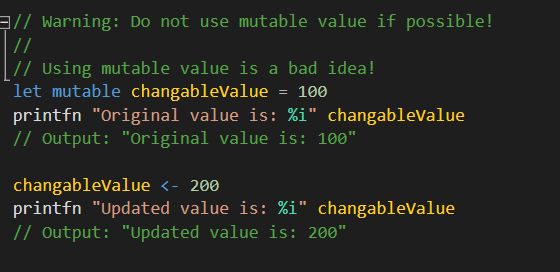
\includegraphics[width=8cm]{pictures/picture02.png}
\end{center}

In addition, if you try to update an immutable/unchangable value using \texttt{<-}, you will get an error. 

\begin{center}
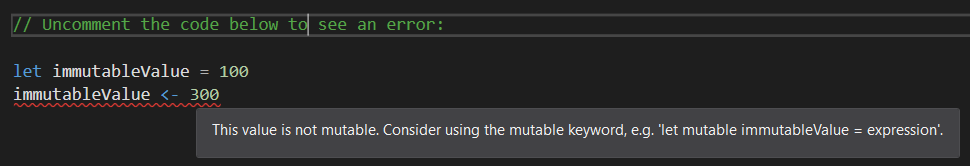
\includegraphics[width=14cm]{pictures/picture03.png}
\end{center}

Why do we recommend immutable/unchangable values: 

Imagine you have a code below, where you have defined a mutable value \texttt{x}, and after thousands of lines of code later, you used \texttt{x}'s value again:

\begin{lstlisting}[language=FSharp]
let mutable x = 100
//
// Thousands of lines of code later......
// You have many lines of code in between......
// It is hard to keep track......
// Have you changed/updated x's value?
// Did you accidentally call any function that modify x?
// Can you guarantee x's value stay unchanged?
// 
//
let y = x + 1
// What is the value of y?
//
// That depends on what happens between y's definition 
// and x's definition.
\end{lstlisting}
\begin{center}
\line(1,0){400}
\end{center}

On the other hand, if \texttt{x} is immutable/unchangable:

\begin{lstlisting}[language=FSharp]
let x = 100
//
// Thousands of lines of code later......
// You have many lines of code in between......
// But because x is immutable/unchangable......
// We can be sure that x stays constant......
// And we can safely conclude that......
//
let y = x + 1
// y = 101
\end{lstlisting}

\pagebreak

\subsubsection{(+) Operator on the same type of variable}

Integers, double, and string support the \texttt{(+)} operation:
\begin{lstlisting}[language=FSharp]

let number1 = 40
let number2 = 55
let addTwoNumbers = number1 + number2

// Remark: "float" and "double" mean the same thing in F#.
let sqrtTwoApprox = 1.414
let piApprox = 3.1415926
let addTwoDecimals = sqrtTwoApprox + piApprox

let sentenceStart = "My school is "
let schoolName = "National University of Singapore"
let combinedSentence = sentenceStart + schoolName
\end{lstlisting}
However, you cannot add an integer with a decimal in F\# directly using \texttt{(+)}, and you cannot add/concatenate a string with a number directly using \texttt{(+)}. If you use VisualStudio, then you may see an error similar to the one below.
\begin{center}
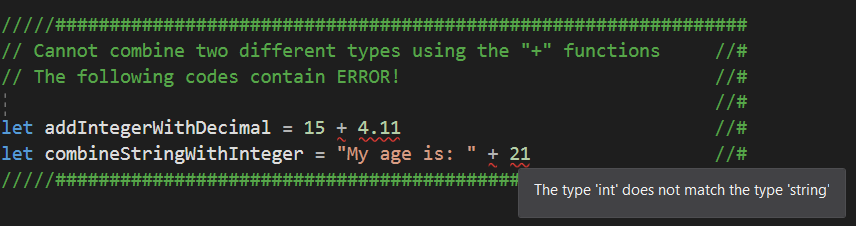
\includegraphics[width=14cm]{pictures/picture04.png}
\end{center}
Furthermore, some functions, like the square root \texttt{sqrt} and math exponent \texttt{(**)} only accepts decimal numbers:

\begin{lstlisting}[language=FSharp]
let sqrtRootOfNine = sqrt 9.0
let twoToPowerOfFive = 2.0 ** 5.0 
\end{lstlisting}
And it will cause error if you use them with integer input instead.
\begin{center}
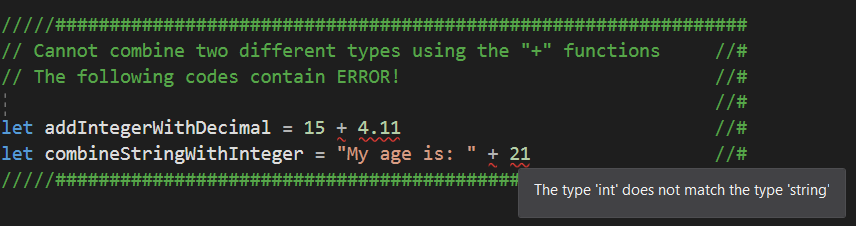
\includegraphics[width=14cm]{pictures/picture04.png}
\end{center}

\pagebreak

\subsubsection{Functions}

\end{document}